\documentclass[a4paper, 14pt]{extarticle}
\usepackage{float}
\usepackage[justification=centering]{caption}
\usepackage{fefutitle}
\usepackage{pythonlisting}
\usepackage{indentfirst}
\usepackage{mathrsfs}
\captionsetup{labelfont=bf, justification=justified}

\begin{document} 
	\fefutitle{1}
	\pagebreak
	\section{Введение}
		В данной лабораторной работе мне нужно реализовать алгоритм построения интегрального преобразования Фурье для произвольно-заданных функций одной переменной.

	\section{Постановка задачи}
	
		Реализовать алгоритм построения интегрального преобразования
		Фурье для произвольно-заданных функций одной переменной. Для реализации потребуются следующие параметры:
		
		\begin{itemize}
			\item \(f(t)\) -- определение функции,
			\item \(a,b\) -- область интегрирования функции,
			\item \(n_1\) -- количество разбиений области интегрирования(также можно использовать шаг \(h_1\)),
			\item \(n_2	\) -- количество разбиений частотного диапазона(также можно использовать шаг \(h_2\)),
			\item \(m\) -- максимальное значение частоты.
		\end{itemize}
	
		Задача сводится к построению спектрального разложения одномерного сигнала \(f(t) \) на частоты составляющих его волн.
		
		Реализация проводится с помощью численных методов расчета
		интегралов. Потребуется построить график функции \(f(t)\), и ее вещественные и комплексные спектральные разложения (\(\mathscr{F_{\Re}}\{f\}\) и \(\mathscr{F_{\Im}}\{f\}\)).
		Графики разложений строятся в диапазоне \(\omega \in [0, m]\). Оси графиков
		разложений представляют из себя по горизонтали -- частотный диапазон, по вертикали -- амплитуда.
		
		Решение оформить в среде \LaTeX.
	
	\section{Решение}
		Рассмотрим функцию \(f(t)=t^2\cdot e^{-4t}\) на диапазоне \([a, b] = [0, 4]\), в остальном диапазоне полагая \(f(t) = 0\). Для аналитического решения, функция примет вид: \( f(t) = t^2\cdot e^{-4t} \cdot \Pi_{0,4}(t) \). Положим \( \chi = 2\pi\omega \). Тогда преобразование Фурье примет вид:
		\begin{align*} \mathscr{F}\big\{t^2\cdot e^{-4t}\big\} &= \int\displaylimits_{-\infty}^{\infty} t^2\cdot e^{-4t} \cdot e^{-i\chi t} \cdot \Pi_{0,4}\;dt = \int\displaylimits_{0}^{4} t^2\cdot e^{-t(4+i\chi)}\;dt = \\ &= - \dfrac{16e^{-16-4i\chi}}{4+i\chi} - \dfrac{8e^{-16-4i\chi}}{(4+i\chi)^2}  - \dfrac{2e^{-16-4i\chi}}{(4+i\chi)^3} + \dfrac{2}{(4+i\chi)^3} \end{align*}
		
		Разложим преобразование на действительную и мнимую части:
		
		\begin{align*}
			\mathscr{F_{\Re}}\big\{t^2\cdot e^{-4t}\big\} &= \cos{4\chi}\cdot e^{-16}\cdot\Bigg(\dfrac{-56}{16+\chi^2} + \dfrac{24\chi^2-128}{(16 + \chi^2)^3}\Bigg) + \\ &+ \chi\sin{4\chi}\cdot e^{-16}\cdot\Bigg(\dfrac{16}{16+\chi^2} + \dfrac{64}{(16+\chi^2)^2} + \dfrac{96 - 2\chi^2}{(16+\chi^2)^3}\Bigg) -\\&- \dfrac{24\chi^2-128}{(16+\chi^2)^3}
		\end{align*}
	
		\begin{align*}
			\mathscr{F_{\Im}}\big\{t^2\cdot e^{-4t}\big\} = \sin{4\chi}\cdot e^{-16}\cdot\Bigg(\dfrac{-56}{16+\chi^2} + \dfrac{24\chi^2-128}{(16 + \chi^2)^3} \Bigg) + \dfrac{96\chi - \chi^3}{(16+\chi^2)^3}
		\end{align*}
		
		В таком случае спектральный график в аналитической форме будет иметь следующий вид :
		\begin{figure}[H]
			\centering
			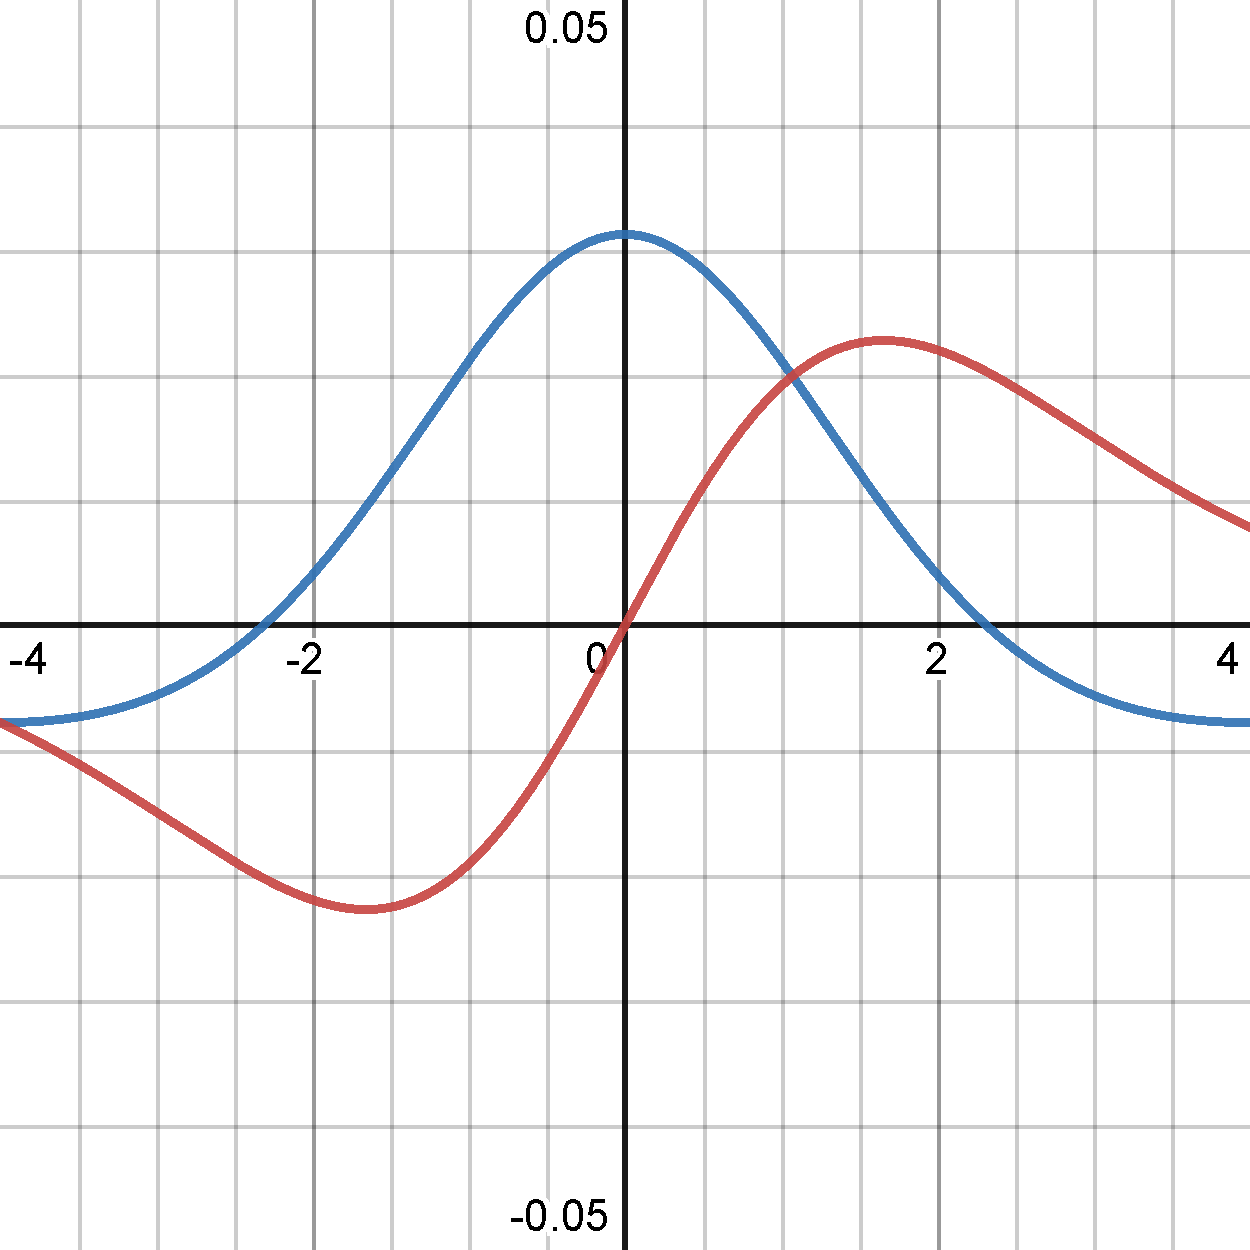
\includegraphics[width = .6\linewidth]{plot1.pdf}
			\caption[.] {Спектральный график волн синус- и косинус-преобразований (красный -- синус, вещественное преобразование, синий -- косинус, комплексное преобразование)}
		\end{figure}
	
		В процессе реализации численного алгоритма, максимальное значение частоты выберем \(m = 2\). Таким образом, численно найденный спектральный график имеет вид:
		\begin{figure}[H]
			\centering
			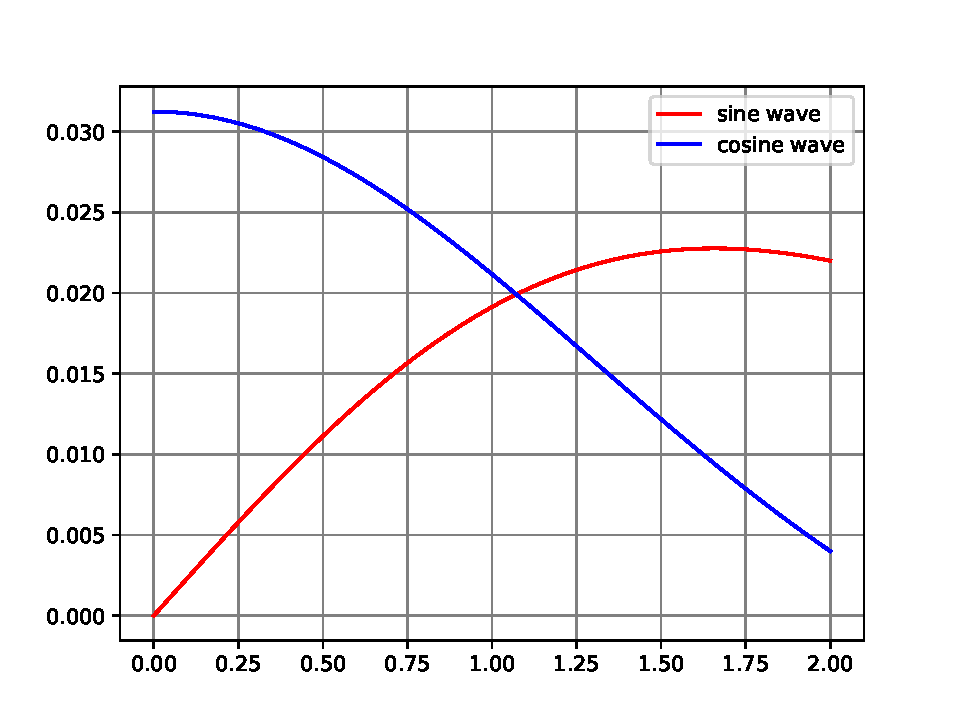
\includegraphics[width = .75\linewidth]{plot2.pdf}
			\caption[.] {Численно рассчитанный спектральный график волн синус- и косинус- преобразований (красный -- синус, синий -- косинус)}
		\end{figure}
	
	\section{Код программы}
		\lstinputlisting[language=Python]{../main.py}
		
	\section{Заключение}
		\noindent Я написал программу на языке <<Python>>, реализующую алгоритм преобразования Фурье. Оформлял отчет по работе  в <<\TeX studio>>.

\end{document}